% !Mode:: "TeX:UTF-8"
%!TEX program  = xelatex

\documentclass[bwprint]{gmcmthesis}
%一个改变表格高度的宏包
\usepackage{array}
%多行公式
\usepackage{amsmath}
\usepackage{amssymb}
%引用图片宏包
\usepackage{caption}
\usepackage{graphicx, subfig}
\usepackage{longtable}
\bibliographystyle{gmcm}
\title{全国研究生数学建模竞赛论文标题}
\baominghao{18102510035} %参赛队号
\schoolname{华东理工大学 \quad 华东师范大学}%学校名称
\membera{沈皓杰} %队员A
\memberb{李佳倩} %队员B
\memberc{张文清} %队员C
\begin{document}
 
 %生成标题
\maketitle
 
 %填写摘要
\begin{abstract}
还没写
\end{abstract}

\pagestyle{plain}

%目录 不推荐加
\tableofcontents
\newpage

\section{问题重述}

\subsection{问题背景}
恐怖袭击是指极端分子或组织人为制造的、针对但不仅限于平民及民用设施的、不符合国际道义的攻击行为。恐怖主义是人类的共同威胁,打击恐怖主义是每个国家应该承担的责任。对恐怖袭击事件相关数据的深入分析有助于加深人们对恐怖主义的认识,为反恐防恐提供有价值的信息支持。
\subsection{需要解决的问题}
现有数据如下:附件1选取了某组织搜集整理的全球恐怖主义数据库(GTD)中1998-2017年世界上发生的恐怖袭击事件的记录;附件2是有关变量的说明,节译自数据库说明文档。附件2文档较长,附件3提供了一个内容摘要。以此3份附件为数据基础,本文依次解决如下问题:

问题1:依据附件1以及其它有关信息,结合现代信息处理技术,借助数学建模方法建立基于数据分析的量化分级模型,将附件1给出的事件按危害程度从高到低分为一至五级,列出近二十年来危害程度最高的十大恐怖袭击事件,并给出表1中事件的分级。

% Table generated by Excel2LaTeX from sheet 'Sheet1'
\renewcommand{\arraystretch}{0.8}
\begin{table}[hbp]%可变参数改变浮动位置的优先级
	\centering
	\caption{典型事件危害级别}
	\begin{tabular}{|c|c|}
		\hline
		\multicolumn{1}{|p{4em}|}{事件编号} & \multicolumn{1}{p{4em}|}{危害级别} \\
		\hline
		200108110012 &  \\
		\hline
		200511180002 &  \\
		\hline
		200901170021 &  \\
		\hline
		201402110015 &  \\
		\hline
		201405010071 &  \\
		\hline
		201411070002 &  \\
		\hline
		201412160041 &  \\
		\hline
		201508010015 &  \\
		\hline
		201705080012 &  \\
		\hline
	\end{tabular}
	\label{tab:addlabel}
\end{table}%
\newpage
问题2:依据事件特征发现恐怖袭击事件制造者。针对在2015、2016年度发生的、尚未有组织或个人宣称负责的恐怖袭击事件,运用数学建模方法寻找并案调查可能性,即将可能是同一个恐怖组织或个人在不同时间、不同地点多次作案的若干案件归为一类,对应的未知作案组织或个人标记不同的代号,并按该组织或个人的危害性从大到小选出其中的前5个,记为1号-5号。再对表2列出的恐袭事件,按嫌疑程度对5个嫌疑人排序,并将结果填入下表(表中样例的意思是:对事件编号为XX的事件,3号的嫌疑最大,其次是4号,最后是5号),如果认为某嫌疑人关系不大,也可以保留空格。
% Table generated by Excel2LaTeX from sheet 'Sheet1'
\renewcommand{\arraystretch}{0.8}
\begin{table}[hbp]
	\centering
	\caption{恐怖份子关于典型事件的嫌疑度}
	\begin{tabular}{|l|l|l|l|l|l|}
		\hline
		\multicolumn{1}{|p{4em}|}{ } & \multicolumn{1}{p{4.7em}|}{1号嫌疑人} & \multicolumn{1}{p{4.7em}|}{2号嫌疑人} & \multicolumn{1}{p{4.7em}|}{3号嫌疑人} & \multicolumn{1}{p{4.7em}|}{4号嫌疑人} & \multicolumn{1}{p{4.7em}|}{5号嫌疑人} \\
		\hline
		\multicolumn{1}{|p{4em}|}{样例XX} & \multicolumn{1}{c|}{4} & \multicolumn{1}{c|}{3} & \multicolumn{1}{c|}{1} & \multicolumn{1}{c|}{2} & \multicolumn{1}{c|}{5} \\
		\hline
		201701090031 &       &       &       &       &  \\
		\hline
		201702210037 &       &       &       &       &  \\
		\hline
		201703120023 &       &       &       &       &  \\
		\hline
		201705050009 &       &       &       &       &  \\
		\hline
		201705050010 &       &       &       &       &  \\
		\hline
		201707010028 &       &       &       &       &  \\
		\hline
		201707020006 &       &       &       &       &  \\
		\hline
		201708110018 &       &       &       &       &  \\
		\hline
		201711010006 &       &       &       &       &  \\
		\hline
		201712010003 &       &       &       &       &  \\
		\hline
	\end{tabular}%
	\label{tab:addlabel}%
\end{table}%

问题3:依据附件1并结合因特网上的有关信息,建立适当的数学模型,研究近三年来恐怖袭击事件发生的主要原因、时空特性、蔓延特性、级别分布等规律,进而分析研判下一年全球或某些重点地区的反恐态势,用图表给出你们的研究结果,提出你们对反恐斗争的见解和建议。

问题4 给出模型和方法,通过数学建模进一步挖掘附件1数据的作用。
\newpage

\section{模型的假设}

\begin{itemize}
\item[假设1] 高维数据(样本)位于一个维数比数据空间维数小得多的流形上;
\item[假设2] 高维数据空间到低维数据空间上的映射是线性映射;
\item[假设3] 不考虑少数样本的特有维度维度对恐怖袭击事件危害程度分级的影响;

\end{itemize}
\newpage

\section{符号说明}

\begin{tabular}{cc}
 \hline
 \makebox[0.4\textwidth][c]{符号}	&  \makebox[0.5\textwidth][c]{意义} \\ \hline
 D	    & 木条宽度(cm) \\ \hline
 L	    & 木板长度(cm)  \\ \hline
 W	    & 木板宽度(cm)  \\ \hline
 N	    & 第n根木条  \\ \hline
 T	    & 木条根数  \\ \hline
 H	    & 桌子高度(cm)  \\ \hline
 R	    & 桌子半径(cm)  \\ \hline
 R	    & 桌子直径(cm)  \\ \hline
\end{tabular}
\newpage

\section{问题一}

\subsection{问题分析}
问题一要求基于附件1给出的恐怖袭击事件记录数据,通过量化分析,将事件按危害程度分级。已知分类信息的历史数据并不完全,因此这是一个典型的数据挖掘聚类问题。

由于附件提供的数据维数很高,数据结构比较复杂,难以将其直观地与恐怖袭击事件的危害程度联系起来。然而对上述数据进行分析时,并非所有属性对随后进行的数据处理都是重要的。高维数据中的信息往往包含在一个或几个低维结构中,可以用少量的简单变量来支配。

因此首先要对数据进行预处理,流程包括数据清理(包括对不完整数据的处理)、数据噪声消除、数据变换(标准化)等。数据经过预处理后,仍保留了其原始的特征和规律,通过主成分分析(Principle Component Analysis,PCA)约减维数可以更好地进行分析。完全定性的聚类方法太过主观;定量聚类方法虽然客观,但由于舍弃了无法量化的信息,会导致结果不符合实际。本文定性与定量相结合,通过基于贝叶斯聚类算法(Bayesian Hierarchical Clustering)的多模块贝叶斯网络方法来进行聚类,最后达到分级的目的。
\subsection{模型建立}
\subsubsection{数据预处理}
首先对全球恐怖主义数据库(GTD)中1998-2017年世界上发生的恐怖袭击事件进行整理,整理步骤如下:

第1步\ 提取确定是恐怖袭击事件的样本;

第2步\ 根据事件摘要来选取与恐怖袭击事件危害程度相关的数据;

第3步\ 将含有缺失数据的样本剔除;

第4步\ 因原数据集中恐怖袭击所致死亡人数和伤亡人数中包含了恐怖分子的死亡和伤亡人数,而本文评估的死伤人数不包含恐怖分子,所以用总的死伤人数分别减去恐怖分子死伤人数得到修正的死亡和伤亡人数;

第5步\ 因第1步和第3步的操作,使得数据集中某些属性的取值不连续,找到这些属性,并将它们的取值连续化。

经过以上整理,得到具有95711条样本量的完整数据集。

\subsubsection{数据降维}
降维是构造降维映射,获得高维数据低维表示的方法,是对大量高维无序且没有明显空间特征数据的处理,以发现隐藏在高维数据中有意义的低维结构。降维问题假设高维数据(样本)位于一个维数比数据空间维数小得多的流形上,降维的目的就是获得这一流形的低维坐标表示。设$\mathit{X}=(x_1,x_2,...x_D)^T$是高维空间$R^D$中的向量,通过降维

\begin{equation}
\mathit{F}(x)=\left( \begin{matrix}{}
\mathit{F}_1(X) \\ 
\mathit{F}_2(X) \\ 
\vdots \\ 
\mathit{F}_d(X)
\end{matrix}\right) =\left( \begin{matrix}{}
\mathit{F}_1(x_1,x_2,\cdots,x_D) \\ 
\mathit{F}_2(x_1,x_2,\cdots,x_D) \\ 
\vdots \\ 
\mathit{F}_d(x_1,x_2,\cdots,x_D)
\end{matrix}\right).
\end{equation}
得到低维空间$\mathit{R}^d$中的向量$\mathit{Y}=(y_1,y_2,\cdots,y_d)^T$。本文假设高维数据到低维空间上的映射是线性映射。因此对于问题一,本文采用主成分分析(Principle Component Analysis,PCA)来进行降维。PCA将数据的主成分(包含信息量大的维度)保留下来,忽略掉对数据描述不重要的成分。即将主成分维度组成的向量空间作为低维空间,将高维数据投影到这个空间上就完成了降维的工作。

设样本数目为$n$,每个样本观测$p$项指标(即维数为$p$)$x_1$,$x_2$,$\cdots$,$x_p$,则根据附件1资料提供的数据标准化处理得到的原始数据矩阵为:
\begin{equation}
\mathit{X}_{np}=\left( \begin{matrix}
	x_{11} & x_{12} & \cdots & x_{1p} \\ 
	x_{21} & x_{22} & \cdots & x_{2p} \\ 
	\vdots & \vdots & \vdots & \vdots \\ 
	x_{n1} & x_{n2} & \cdots & x_{np}
\end{matrix}\right) \equiv \left(
\begin{matrix}
\mathit{X}_1 & \mathit{X}_2 & \cdots & \mathit{X}_p
\end{matrix} 
\right).  
\end{equation}
用数据矩阵$\mathit{X}_{np}$的$p$个向量$\mathit{X}_1$,$\mathit{X}_2$,$\mathit{X}_p$作线性组合为:

\begin{equation}
\mathit{F}_i=a_{i1}\mathit{X}_1+a_{i2}\mathit{X}_2+\cdots+a_{ip}\mathit{X}_p(i=1,2,\cdots,p).
\label{1} 
\end{equation}

其中,系数$a_{ij}$由下列原则来确定:

1.$\mathit{F}_i$与$\mathit{F}_j$互不相关。

2.$\mathit{F}_1$是$x_1$,$x_2$,$\cdots$,$x_p$的一切线性组合且满足(\ref{1})中方差最大的;$\mathit{F}_2$是与$\mathit{F}_1$不相关的$x_1$,$x_2$,$\cdots$,$x_p$的所有线性组合中方差最大者;$\mathit{F}_p$是与$\mathit{F}_1$,$\mathit{F}_2$,$\cdots$,$\mathit{F}_{p-1}$都不相关的$x_1$,$x_2$,$\cdots$,$x_p$的一切线性组合中方差最大的。


根据定理,由$\mathit{X}$求得的协方差矩阵就是相关系数矩阵
\begin{equation}
	\mathit{A}=\left(\begin{matrix}
	a_{11} & a_{12} & \cdots & a_{1p} \\ 
	a_{21} & a_{22} & \cdots & a_{2p} \\ 
	\vdots & \vdots & \vdots & \vdots \\ 
	a_{p1} & a_{p2} & \cdots & a_{pp}
	\end{matrix} \right).
\end{equation}

求$A$的特征值和特征向量可通过正交变换$T$使
\begin{equation}
	T^{-1}AT=\left(\begin{matrix}
	\lambda_1 &  &  &  \\ 
	& \lambda_2 &  &  \\ 
	&  & \ddots &  \\ 
	&  &  & \lambda_p
	\end{matrix}  \right). 
\end{equation}

按照累积方差贡献率$\frac{\sum_{j=1}^k\lambda_j}{\sum_{j=1}^pr_{jj}}= \dfrac{\sum_{j=1}^k\lambda_j}{p}>85\%$从而建立前$k$个主成分:
\begin{equation}
\mathit{F}_i=a_{i1}\mathit{X}_1+a_{i2}\mathit{X}_2+\cdots+a_{ip}\mathit{X}_p(i=1,2,\cdots,k).
\end{equation}

\subsubsection{数据聚类}
本文将用于恐怖袭击危害程度分级的贝叶斯网络分为4个模块,分别是恐怖袭击危害程度的分级贝叶斯网络模块以及3个后果子模块:财产损失模块、人员伤亡模块和不良社会影响模块。图\ref{分级贝叶斯网络模块}是恐怖袭击危害程度的分级贝叶斯网络模块,其中的置换节点可以被相应的贝叶斯网络模块所置换。HL(harm level)表示危害程度,PD(property damage)和CeP(casualties except perpetrators)是恐怖主义活动造成财产损失和人员伤亡情况,并且人员伤亡不包括恐怖份子。ASI(adverse social impacts)是恐怖主义行为造成的社会不良影响程度。
\begin{figure}[!h]
	\centering
	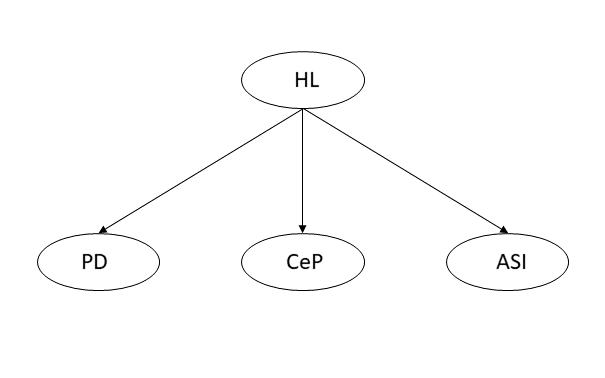
\includegraphics[width=.7\textwidth]{1.png}
	\caption{分级贝叶斯网络模块}
	\label{分级贝叶斯网络模块}
\end{figure}

由于财产损失模块和人员伤亡模块的样本数据具有特征(feature)和标签(label)。因此对于这2个模块,我们采用监督学习的方法来构建,本质上就是找到特征和标签间的映射。对于不良社会影响模块,根据专家知识来构建较为合理。

本文先对人员伤亡贝叶斯网络模块的构建进行分析,财产损失的构建方法类似。人员伤亡贝叶斯网络模块中的节点,表示对人员伤亡评估有意义的情报信息或者经过情报机构的专业人员通过数据融合获得的信息。表\ref{贝叶斯网络结构中的节点变量说明}表示对于人员伤亡模块,有人员伤亡1个类节点和15个属性节点。
%\begin{longtable}[!hbt]
%	\centering
%	\caption{贝叶斯网络结构中的节点变量说明}
%	\toprule  %添加表格头部粗线
%	node ID& node name& node size& node value\\
%	\midrule  %添加表格中横线
%	1& date& 2& 1=双休日\\
%	&&& 0=工作日\\
%	2& country& & 采用ISO国际标准国家代码,见附录\\
%	3& region& 12& 1=北美\\
%	&&& 2=中美洲和加勒比海地区\\
%	&&& 3=南美\\
%	&&& 4=东亚\\
%	&&& 5=东南亚\\
%	&&& 6=南亚\\
%	&&& 7=中亚\\
%	&&& 8=西欧\\
%	&&& 9=东欧\\
%	&&& 10=中东和北非\\
%	&&& 11=撒哈拉以南的非洲\\
%	&&& 12=澳大利亚和大洋洲\\
%	4& crit1(政治、经济、宗教或社会目标)& 2&  1=“是”事件满足标准1\\
%	&&& 0=“否”事件不满足标准1或者没有明确表明满足标准1\\
%	5& cite2(意图胁迫、恐吓或煽动更多的群众)& 2& 1=“是”事件满足标准1\\
%	&&& 0=“否”事件不满足标准1或者没有明确表明满足标准1\\
%	6& cite3(超出国际人道主义法律范围)& 2& 1=“是”事件满足标准1\\
%	&&& 0=“否”事件不满足标准1或者没有明确表明满足标准1\\
%	7& success(成功的攻击)& 12& 1=“是”这一事件是成功的\\
%	&&& 0=“否”这一事件不成功的\\
%	8& suicide(自杀式袭击)& 2& 1=“是”这一事件是自杀式袭击\\
%	&&& 0=“否”没有任何迹象表明,该事件是一个自杀式袭击\\
%	9& attacktype& 9& 1=暗杀\\
%	&&& 2=武装袭击\\
%	&&& 3=轰炸/爆炸\\
%	&&& 4=劫持\\
%	&&& 5=劫持人质(路障事件)\\
%	&&& 6=劫持人质(绑架)\\
%	&&& 7=设施/基础设施攻击\\
%	&&& 8=徒手攻击\\
%	&&& 9=未知\\
%	10& targtype& 22& 1=商业\\
%	&&& 2=政府(一般意义)\\
%	&&& 3=警察\\
%	&&& 4=军事\\
%	&&& 5=流产有关\\
%	&&& 6=机场和飞机\\
%	&&& 7=政府(外交)\\
%	&&& 8=教育机构\\
%	&&& 9=食物或水供应\\
%	&&& 10=新闻记者\\
%	&&& 11=海事(包括港口和海上设施)\\
%	&&& 12=非政府组织(NGO) \\
%	&&& 13=其他\\
%	&&& 14=公民自身和私有财产\\
%	&&& 15=宗教人物/机构\\
%	&&& 16=电信\\
%	&&& 17=恐怖分子/非州立民兵组织\\
%	&&& 18=游客\\
%	&&& 19=运输(航空除外)\\
%	&&& 20=未知\\
%	&&& 21=公用事业\\
%	&&& 22=暴力政党\\
%	11& weaptype& 13& 1=生物武器\\
%	&&& 2=化学武器\\
%	&&& 3=放射性武器\\
%	&&& 4=核武器\\
%	&&& 5=轻武器\\
%	&&& 6=爆炸物/炸弹/炸药\\
%	&&& 7=假武器\\
%	&&& 8=燃烧武器\\
%	&&& 9=致乱武器\\
%	&&& 10=交通工具\\
%	&&& 11=破坏设备\\
%	&&& 12=其他\\
%	&&& 13=未知\\
%	12& kill& n& n=死亡总人数减去凶手死亡人数\\
%	13& wound& n& n=受伤总人数减去凶手受伤人数\\
%	14& propexten(财产损害程度)& 4& 1=灾难性的\\
%	&&& 2=重大的\\
%	&&& 3=较小的\\
%	&&& 4=未知\\
%	15& extended(持续事件)& 2& 1=“是”事件的持续时间达到24个小时以上\\
%	&&& 0=“否”事件的持续时间不到24小时\\
%	\bottomrule %添加表格底部粗线
%	\label{贝叶斯网络结构中的节点变量说明}
%\end{longtable} 
	

对于本文的人员伤亡模块,其节点变量较少,所以文本用打分搜索方法中的K2算法来构建贝叶斯网络。这个算法需要指定结点的先验顺序。节点顺序主要包括领域知识或节点偏序指定的约束。为了确定唯一的初始节点序,我们首先基于定向后的最大权重跨度树对节点块排序,结点块的排序是唯一的,然后再采用局部完全有向无环图法对块内节点排序,最终得到所有节点的排序结构如图。同理可得财产损失模块的贝叶斯网络结构如图所示。

其次对不良社会影响模块进行分析。根据专家知识可知,恐怖袭击事件造成的不良社会影响跟恐怖袭击事件造成的人员伤亡、财产损失,恐怖主义活动发生前是否威胁、恐吓或向大众传播某种恐怖消息,以及民众或反恐决策人员对恐怖袭击的知情程度密切相关。由此得到图\ref{不良社会影响模块的贝叶斯网络结构}所示的不良社会影响模块的贝叶斯网络结构。TA(terrorist atmosphere)是恐怖份子是否在恐怖活动前对大众造成恐吓或威胁;DK(degree of knowledge)是民众对恐怖袭击的知情程度。PD和TA的状态合集如\ref{不良社会影响模块}所示。根据专家知识,ASI,CeP和DK变量的状态合集如表:

\begin{figure}[!h]
	\centering
	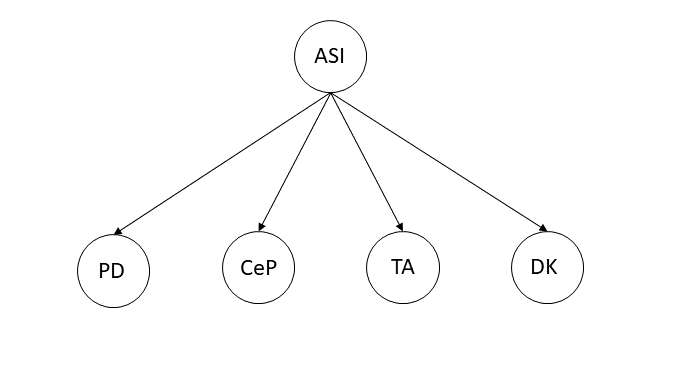
\includegraphics[width=.7\textwidth]{2.png}
	\caption{不良社会影响模块的贝叶斯网络结构}
	\label{不良社会影响模块的贝叶斯网络结构}
\end{figure}
%\begin{table}[!hbt]
%	\centering
%	\begin{ tabular }{p{2cm}<{\centering}p{4cm}<{\centering}p{2cm}<{\centering}p{4cm}<{\centering}}%{cccc}
%		\toprule  %添加表格头部粗线
%		node ID& node name& node size& node value\\
%		\midrule  %添加表格中横线
%		1& ASI& 4& 1=Minimal\\
%		&&& 2=Minor\\
%		&&& 3=Major\\
%		&&& 4=Catastrophic\\
%		2& CeP& 5& 1=None\\
%		&&& 2= Minimal (1≦nkill<3 or 1≦nwound<10)\\
%		&&& 3=Minor (3≦nkill<10 or 10≦nwound<50)\\
%		&&& 4= Major (10≦nkill<30 or 30≦nwound<50) \\
%		&&& 5= Catastrophic (nkill≧30 or nwound≧50) \\
%		3& DK& 4& 1= Minimal \\
%		&&& 2= Minor \\
%		&&& 3= Major \\
%		&&& 4= Catastrophic \\
%		\bottomrule %添加表格底部粗线
%	\end{ tabular }
%	\label{不良社会影响模块}
%\end{table} 


设贝叶斯网络中某一节点$R$,它有$n$个取值,每个取值的先验概率为$p(r_i)$,且$\sum_{i=1}^np(r_i)=1$,节点$R$有一取$m$个值的子节点$S$,$p(S|R)$的条件概率矩阵为
\begin{equation}
	P=\left( \begin{matrix}
	p_{11} & p_{12} & \cdots & p_{1m} \\ 
	p_{21} & p_{22} & \cdots & p_{2m} \\ 
	\vdots & \vdots & \ddots & \vdots \\ 
	p_{n1} & p_{n2} & \cdots & p_{nm}
	\end{matrix} \right).
\end{equation}

财产损失模块和人员伤亡模块贝叶斯网络,由于存在观测数据,可以从数据中学习参数的概率分布表,但没有与分级贝叶斯网络和不良社会影响模块贝叶斯网络相关的观测数据,所以这2个贝叶斯网络模块的概率分布表采用主观赋权法来确定。
考虑多个专家给出$p(S|R)$的条件概率矩阵为
\begin{equation}
P^k=\left( \begin{matrix}
p_{11} & p_{12} & \cdots & p_{1m} \\ 
p_{21} & p_{22} & \cdots & p_{2m} \\ 
\vdots & \vdots & \ddots & \vdots \\ 
p_{n1} & p_{n2} & \cdots & p_{nm}
\end{matrix} \right).
\end{equation}

其中$k=1,2,\cdots,q$表示专家的个数,设每个专家的权重为$H=(h_1,h_2,\cdots,h_q)^T$,其中$\sum_{k=1}^qh_k=1$.为了确定各条件概率值,建立优化模型:

%谁来搞一下这个公式
%\begin{gather}
%\min L=\sum_{i=1}^np(a_i)\sum_{k=1}^q\sum_{j=1}^mh_k(p_{ij}-{p_{ij}^k)^2 \notag\\
%	s.t\quad\sum_{j=1}^mp_{ij}=1(i=1,2,\cdots,n)\notag\\
%	p_{ij}\ge\bigtriangleup 0(i=1,2,\cdots,n;j=1,2,\cdots,m)\\
%\end{gather}
%\begin{center}
%\begin{equation} \label{eqn3}
%\begin{split}
%\min\slL&=\sum\limits_{i=1}^{n}p(a_i) \sum\limits_{k=1}^{q}\sum\limits_{j=1}^{m}h_k(p_i_j- p_{ij}^k)^2\\
%\mathrm{s.t.}\sum\limits_{j=1}^{m}p_i_j&=1(i=1,2,\cdots,n),\\
%p_i_j\geq 0(i=1,2,\cdots,n;j=i=1,2,\cdots,m)
%\end{split}
%\end{equation}
%\end{center}



该优化模型的目标是使条件概率矩阵与专家给出的条件概率之间的总偏差平方和最小。由$\frac{\partial L}{\partial p_{ij}}$得条件概率的主观概率为
\begin{equation}
	p_{ij}=\sum_{k=1}^{q}h_kp_{ij}^k(i=1,2,\cdots,n;j=1,2,\cdots,m).
\end{equation}
\subsection{问题求解}
贝叶斯网络推理是概率分布的计算过程,即在给定模型中计算目标变量的后验概率。根据本文的多模块贝叶斯网络,可以从观测的事件出发逐层推理,得到置换节点的状态,最后推理得到恐怖袭击威胁等级。本文的多模块贝叶斯网络差异较大,因此针对不同的模块,本文选择不同的推理算法。对于分级贝叶斯网络模块,本文采用多树传播推理算法;其他3个贝叶斯网络模块采用联结树推理算法。联结树算法将有向图转换为树,从而大大减小了计算的复杂度,计算速度较快并且适用性强,对网络中存在多个查询节点进行推理时非常便捷。本文先将贝叶斯网络转化为联结树,然后对联结树上的消息传递过程进行定义,再计算概率,基本过程如下:

1、建立Moral图:将有向图转换为无向图,找出每个节点的父节点并连接起来把所有的有向边改为无向边

2、将Moral图三角化:三角化是指让图中不存在超过3个点的环。将大于等于4的环,取其中两个非相邻节点用无向边连接起来,进行Moral图的三角化,即对顶点的一一删除。具体规则为(1)成对的联结该顶点的相邻节点;(2)删除该节点,并添加边;(3)删除的顶点必须保证,所需要添加的边最少。

3、在三角化的图中确定团:每个三角都代表了一个节点,两个相临的三角具有共同的边。这条边就成为两个节点之间的中间节点。如此就组成一张联通图。找到三角化后Moral图中构成联结树的所有团,团即为最大全联通子图,其中每对不同节点都有边相连。

4.建立联结树
\section{问题二}

\section{问题三}
\section{问题四}



%参考文献   手工录入
%\begin{thebibliography}{9}%宽度9
% \bibitem{bib:one} ....
% \bibitem{bib:two} ....
%\end{thebibliography}

%采用bibtex方案

%\cite{mittelbach_latex_2004,wright_latex3_2009,beeton_unicode_2008,vieth_experiences_2009}
\bibliography{example}

\newpage
%附录
\appendix
%\setcounter{page}{1} %如果需要可以自行重置页码。
\section{我的 MATLAB 源程序}
\begin{lstlisting}[language=MATLAB]%设置不同语言即可。
kk=2;[mdd,ndd]=size(dd);
while ~isempty(V)
[tmpd,j]=min(W(i,V));tmpj=V(j);
for k=2:ndd
[tmp1,jj]=min(dd(1,k)+W(dd(2,k),V));
tmp2=V(jj);tt(k-1,:)=[tmp1,tmp2,jj];
end
tmp=[tmpd,tmpj,j;tt];[tmp3,tmp4]=min(tmp(:,1));
if tmp3==tmpd, ss(1:2,kk)=[i;tmp(tmp4,2)];
else,tmp5=find(ss(:,tmp4)~=0);tmp6=length(tmp5);
if dd(2,tmp4)==ss(tmp6,tmp4)
ss(1:tmp6+1,kk)=[ss(tmp5,tmp4);tmp(tmp4,2)];
else, ss(1:3,kk)=[i;dd(2,tmp4);tmp(tmp4,2)];
end;end
dd=[dd,[tmp3;tmp(tmp4,2)]];V(tmp(tmp4,3))=[];
[mdd,ndd]=size(dd);kk=kk+1;
end; S=ss; D=dd(1,:);


 \end{lstlisting}


\end{document} 